\section{Double integrals}
\subsection{In Cartesian coordinates ($x,y$)}
\tableofcontents[currentsection,currentsubsection]
\iffalse
\begin{frame}{Double integrals (intuition)}
    Sometimes we need to take an integral over a integral.
    This is useful for example when calculating the volume of a 3D body.
    \begin{itemize}
        \item \textbf{Question:} calculate the volume of the 3D body between $z=f(x,y)=(2x+3)e^y$ and the $xy$-plane, when the bounds of $x$ and $y$ are the rectangle $-1\leq x\leq1$ and $0\leq y\leq2$.
        \item \textbf{Intuition:} the volume consists of a large number of very small ``boxes'' (3D-rectangles). The volume of one such ``box" is $\text{length}\cdot\text{width}\cdot\text{height}=dx\cdot dy\cdot(2x+3)e^y$. The total volume of the 3D body must be the sum of all these little boxes, i.e., an integral:
            \[V_{\text{tot}}=\int_{0}^{2}\int_{-1}^{1}(2x+3)e^y dxdy=\int_{-1}^{1}\int_{0}^{2}(2x+3)e^y dydx\]
        The next slides cover how to compute such a double integral.
    \item    \textbf{Note:} in the case of a rectangle, the order of integration does not matter (that's why the two double integals above are equivalent).
    \end{itemize}
\end{frame}
\fi


\begin{frame}{Computing normal double integrals (1/2)}
    \footnotesize
    \begin{itemize}
        \item \textbf{Question:} calculate the volume of the 3D body between $z=f(x,y)=(2x+3)e^y$ and the $xy$-plane, when the bounds of $x$ and $y$ are the rectangle $-1\leq x\leq1$ and $0\leq y\leq2$.
        \item\pause The region of integration is $D=\{(x,y)\mid-1\leq x\leq1,~ 0\leq y\leq2\}=[-1,1]\times[0,2]$
        \item\pause We need to compute the double integral\footnote{The reverse order would also work:
            $V_{\text{tot}}=\int_{-1}^{1}\red{\int_{0}^{2}(2x+3)e^y dy}dx$}
            \[V_{\text{tot}}=\int_{0}^{2}\red{\int_{-1}^{1}(2x+3)e^y dx}dy\]
        \item\pause \textbf{Plan of attack:} work from the inside-out. So, we start solving the inner integral: $\red{\int_{-1}^{1}(2x+3)e^y dx}$. \textbf{Important:} this is an integral in the ``$x$-world", because of the $dx$. It means that $x$ changes, whereas we can treat $y$ as a constant when computing the integral. So:
            \[\red{\int_{-1}^{1}(2x+3)e^y dx}=e^y\int_{-1}^1(2x+3)dx=e^y\left[x^2+3x\right]_{-1}^1=6e^y\]
    \end{itemize}
\end{frame}

\begin{frame}{Computing normal double integrals (2/2)}
    \begin{itemize}
        \item \textbf{Question:} calculate the volume of the 3D body between $z=f(x,y)=(2x+3)e^y$ and the $xy$-plane, when the bounds of $x$ and $y$ are the rectangle $-1\leq x\leq1$ and $0\leq y\leq2$.
            \[V_{\text{tot}}=\int_{0}^{2}\blue{\int_{-1}^{1}(2x+3)e^y dx}dy\]
        \item\pause We found:
            \[\blue{\int_{-1}^{1}(2x+3)e^y dx}=\red{6e^y}\]
        \item\pause We substitute this into the original double integral:
            \[V_{\text{tot}}=\int_{0}^{2}\red{6e^y}dy=6\left[e^y\right]_0^2=6e^2-6\]
        \item\pause \textbf{Conclusion:} the volume of the 3D body is $\boxed{V_{\text{tot}}=6e^2-6}$.
    \end{itemize}
\end{frame}


\begin{frame}{Another straightforward double integral}
    \begin{itemize}
        \item \textbf{Question:} calculate the volume of the 3D body between $z=f(x,y)=\frac{x^3}{y}$ and the $xy$-plane, when the bounds of $x$ and $y$ are the rectangle $3\leq x\leq5$ and $2\leq y\leq4$.
        \item\pause We want to solve the integral
            \[\int_2^4\int_3^5\frac{x^3}{y}dxdy\]
            We start with solving the inner integral, where $x$ changes and $y$ is constant:
            \[\int_3^5\frac{x^3}{y}dx=\frac{1}{y}\int_3^5x^3dx=\frac{1}{4y}\left[x^4\right]_3^5=\frac{136}{y}\]
            \pause Now we calculate the full double integral: the volume is
            \[\int_2^4\int_3^5\frac{x^3}{y}dxdy=\int_2^4\frac{136}{y}dy=136\left[\ln y\right]_2^4=\boxed{136\ln2}\]
    \end{itemize}
\end{frame}

\begin{frame}{General regions: Intuition}
    



\tikzset{every picture/.style={line width=0.75pt}} %set default line width to 0.75pt        

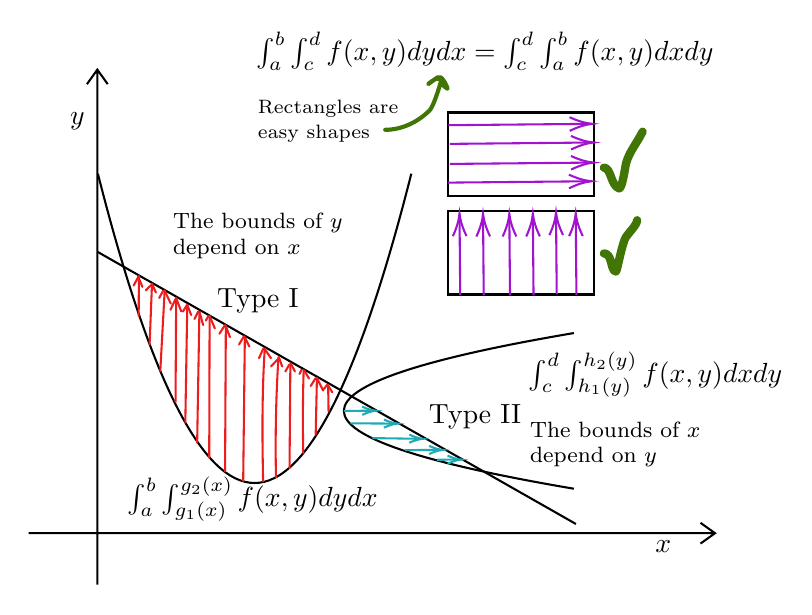
\begin{tikzpicture}[x=0.75pt,y=0.75pt,yscale=-1,xscale=1]
%uncomment if require: \path (0,300); %set diagram left start at 0, and has height of 300

%Shape: Axis 2D [id:dp15786148290852164] 
\draw  (66.67,256.35) -- (397.33,256.35)(99.73,33) -- (99.73,281.17) (390.33,251.35) -- (397.33,256.35) -- (390.33,261.35) (94.73,40) -- (99.73,33) -- (104.73,40)  ;
%Shape: Parabola [id:dp3374340259040851] 
\draw   (100,83.17) .. controls (150.33,281.83) and (200.67,281.83) .. (251,83.17) ;
%Straight Lines [id:da17471303708405084] 
\draw    (100,120.89) -- (330.33,251.92) ;
%Shape: Free Drawing [id:dp969312824964295] 
\draw  [color={rgb, 255:red, 237; green, 29; blue, 29 }  ,draw opacity=1 ][line width=0.75] [line join = round][line cap = round] (119.65,151.75) .. controls (119.68,145.3) and (119.72,138.84) .. (119.75,132.39) ;
%Shape: Free Drawing [id:dp25577323232811455] 
\draw  [color={rgb, 255:red, 237; green, 29; blue, 29 }  ,draw opacity=1 ][line width=0.75] [line join = round][line cap = round] (119.33,132.6) .. controls (120.04,134.28) and (120.74,135.96) .. (121.44,137.65) ;
%Shape: Free Drawing [id:dp5698702687630868] 
\draw  [color={rgb, 255:red, 237; green, 29; blue, 29 }  ,draw opacity=1 ][line width=0.75] [line join = round][line cap = round] (119.54,132.7) .. controls (118.77,134.14) and (118,135.58) .. (117.23,137.02) ;
%Shape: Free Drawing [id:dp29855586454232697] 
\draw  [color={rgb, 255:red, 237; green, 29; blue, 29 }  ,draw opacity=1 ][line width=0.75] [line join = round][line cap = round] (124.91,165.44) .. controls (125.3,155.68) and (125.68,145.93) .. (126.07,136.18) ;
%Shape: Free Drawing [id:dp5518305641486789] 
\draw  [color={rgb, 255:red, 237; green, 29; blue, 29 }  ,draw opacity=1 ][line width=0.75] [line join = round][line cap = round] (126.07,136.18) .. controls (126.7,137.58) and (127.33,138.98) .. (127.96,140.39) ;
%Shape: Free Drawing [id:dp3337563336556728] 
\draw  [color={rgb, 255:red, 237; green, 29; blue, 29 }  ,draw opacity=1 ][line width=0.75] [line join = round][line cap = round] (126.07,136.39) .. controls (125.09,137.37) and (124.11,138.35) .. (123.12,139.33) ;
%Shape: Free Drawing [id:dp7548434878361339] 
\draw  [color={rgb, 255:red, 237; green, 29; blue, 29 }  ,draw opacity=1 ][line width=0.75] [line join = round][line cap = round] (130.07,178.07) .. controls (130.77,165.23) and (131.47,152.39) .. (132.18,139.54) ;
%Shape: Free Drawing [id:dp3798761747267194] 
\draw  [color={rgb, 255:red, 237; green, 29; blue, 29 }  ,draw opacity=1 ][line width=0.75] [line join = round][line cap = round] (132.18,139.54) .. controls (133.16,141.61) and (134.14,143.68) .. (135.12,145.75) ;
%Shape: Free Drawing [id:dp032826386853152645] 
\draw  [color={rgb, 255:red, 237; green, 29; blue, 29 }  ,draw opacity=1 ][line width=0.75] [line join = round][line cap = round] (131.44,139.54) .. controls (130.81,140.7) and (130.18,141.86) .. (129.54,143.02) ;
%Shape: Free Drawing [id:dp03973270620885261] 
\draw  [color={rgb, 255:red, 237; green, 29; blue, 29 }  ,draw opacity=1 ][line width=0.75] [line join = round][line cap = round] (137.4,193.12) .. controls (137.51,176.39) and (137.61,159.65) .. (137.72,142.91) ;
%Shape: Free Drawing [id:dp5585733615581354] 
\draw  [color={rgb, 255:red, 237; green, 29; blue, 29 }  ,draw opacity=1 ][line width=0.75] [line join = round][line cap = round] (137.72,143.12) .. controls (138.53,145.23) and (139.33,147.33) .. (140.14,149.44) ;
%Shape: Free Drawing [id:dp09502119147890964] 
\draw  [color={rgb, 255:red, 237; green, 29; blue, 29 }  ,draw opacity=1 ][line width=0.75] [line join = round][line cap = round] (137.51,143.33) .. controls (136.67,145.12) and (135.82,146.91) .. (134.98,148.7) ;
%Shape: Free Drawing [id:dp5291512546852979] 
\draw  [color={rgb, 255:red, 237; green, 29; blue, 29 }  ,draw opacity=1 ][line width=0.75] [line join = round][line cap = round] (142.12,202.98) .. controls (142.43,184.12) and (142.75,165.25) .. (143.06,146.39) ;
%Shape: Free Drawing [id:dp5772349371864574] 
\draw  [color={rgb, 255:red, 237; green, 29; blue, 29 }  ,draw opacity=1 ][line width=0.75] [line join = round][line cap = round] (143.06,146.39) .. controls (143.69,148) and (144.31,149.61) .. (144.94,151.22) ;
%Shape: Free Drawing [id:dp1972925958236551] 
\draw  [color={rgb, 255:red, 237; green, 29; blue, 29 }  ,draw opacity=1 ][line width=0.75] [line join = round][line cap = round] (142.94,146.39) .. controls (142.27,147.45) and (141.61,148.51) .. (140.94,149.57) ;
%Shape: Free Drawing [id:dp8420460315730172] 
\draw  [color={rgb, 255:red, 237; green, 29; blue, 29 }  ,draw opacity=1 ][line width=0.75] [line join = round][line cap = round] (147.82,212.79) .. controls (148.18,191.76) and (148.55,170.73) .. (148.91,149.7) ;
%Shape: Free Drawing [id:dp27970958158007964] 
\draw  [color={rgb, 255:red, 237; green, 29; blue, 29 }  ,draw opacity=1 ][line width=0.75] [line join = round][line cap = round] (148.91,149.7) .. controls (149.52,151.82) and (150.12,153.94) .. (150.73,156.06) ;
%Shape: Free Drawing [id:dp5649824516326716] 
\draw  [color={rgb, 255:red, 237; green, 29; blue, 29 }  ,draw opacity=1 ][line width=0.75] [line join = round][line cap = round] (148.36,149.52) .. controls (147.76,150.73) and (147.15,151.94) .. (146.55,153.15) ;
%Shape: Free Drawing [id:dp3968145714534206] 
\draw  [color={rgb, 255:red, 237; green, 29; blue, 29 }  ,draw opacity=1 ][line width=0.75] [line join = round][line cap = round] (153.64,220.06) .. controls (153.7,197.27) and (153.76,174.48) .. (153.82,151.7) ;
%Shape: Free Drawing [id:dp6978169307097055] 
\draw  [color={rgb, 255:red, 237; green, 29; blue, 29 }  ,draw opacity=1 ][line width=0.75] [line join = round][line cap = round] (153.82,151.7) .. controls (154.67,153.7) and (155.52,155.7) .. (156.36,157.7) ;
%Shape: Free Drawing [id:dp8965668318145716] 
\draw  [color={rgb, 255:red, 237; green, 29; blue, 29 }  ,draw opacity=1 ][line width=0.75] [line join = round][line cap = round] (153.27,151.7) .. controls (152.85,152.42) and (152.42,153.15) .. (152,153.88) ;
%Shape: Free Drawing [id:dp973778437675962] 
\draw  [color={rgb, 255:red, 237; green, 29; blue, 29 }  ,draw opacity=1 ][line width=0.75] [line join = round][line cap = round] (161.27,226.61) .. controls (161.39,203.21) and (161.52,179.82) .. (161.64,156.42) ;
%Shape: Free Drawing [id:dp8382224187332488] 
\draw  [color={rgb, 255:red, 237; green, 29; blue, 29 }  ,draw opacity=1 ][line width=0.75] [line join = round][line cap = round] (161.64,156.61) .. controls (162.3,158.36) and (162.97,160.12) .. (163.64,161.88) ;
%Shape: Free Drawing [id:dp7905567713416519] 
\draw  [color={rgb, 255:red, 237; green, 29; blue, 29 }  ,draw opacity=1 ][line width=0.75] [line join = round][line cap = round] (161.27,156.06) .. controls (160.36,157.45) and (159.45,158.85) .. (158.55,160.24) ;
%Shape: Free Drawing [id:dp29787258326310195] 
\draw  [color={rgb, 255:red, 237; green, 29; blue, 29 }  ,draw opacity=1 ][line width=0.75] [line join = round][line cap = round] (170,231.23) .. controls (170.27,208.1) and (170.53,184.97) .. (170.8,161.83) ;
%Shape: Free Drawing [id:dp9274205944195231] 
\draw  [color={rgb, 255:red, 237; green, 29; blue, 29 }  ,draw opacity=1 ][line width=0.75] [line join = round][line cap = round] (170.8,162.03) .. controls (171.53,163.5) and (172.27,164.97) .. (173,166.43) ;
%Shape: Free Drawing [id:dp7693301223812206] 
\draw  [color={rgb, 255:red, 237; green, 29; blue, 29 }  ,draw opacity=1 ][line width=0.75] [line join = round][line cap = round] (170.4,161.43) .. controls (169.6,162.77) and (168.8,164.1) .. (168,165.43) ;
%Shape: Free Drawing [id:dp7782707170438627] 
\draw  [color={rgb, 255:red, 237; green, 29; blue, 29 }  ,draw opacity=1 ][line width=0.75] [line join = round][line cap = round] (179.6,231.43) .. controls (179.17,210.1) and (179.02,188.72) .. (180.4,167.43) ;
%Shape: Free Drawing [id:dp49133737965272806] 
\draw  [color={rgb, 255:red, 237; green, 29; blue, 29 }  ,draw opacity=1 ][line width=0.75] [line join = round][line cap = round] (180.4,167.63) .. controls (181.4,169.1) and (182.4,170.57) .. (183.4,172.03) ;
%Shape: Free Drawing [id:dp0785267232113096] 
\draw  [color={rgb, 255:red, 237; green, 29; blue, 29 }  ,draw opacity=1 ][line width=0.75] [line join = round][line cap = round] (179.8,167.23) .. controls (179.07,168.83) and (178.33,170.43) .. (177.6,172.03) ;
%Shape: Free Drawing [id:dp037346878597830147] 
\draw  [color={rgb, 255:red, 237; green, 29; blue, 29 }  ,draw opacity=1 ][line width=0.75] [line join = round][line cap = round] (185.8,229.43) .. controls (185.41,210.17) and (185.77,190.86) .. (187,171.63) ;
%Shape: Free Drawing [id:dp35237958666754987] 
\draw  [color={rgb, 255:red, 237; green, 29; blue, 29 }  ,draw opacity=1 ][line width=0.75] [line join = round][line cap = round] (187.2,171.63) .. controls (187.73,173.1) and (188.27,174.57) .. (188.8,176.03) ;
%Shape: Free Drawing [id:dp7470758145524414] 
\draw  [color={rgb, 255:red, 237; green, 29; blue, 29 }  ,draw opacity=1 ][line width=0.75] [line join = round][line cap = round] (186.8,172.43) .. controls (185.67,173.63) and (184.53,174.83) .. (183.4,176.03) ;
%Shape: Free Drawing [id:dp018728777026371768] 
\draw  [color={rgb, 255:red, 237; green, 29; blue, 29 }  ,draw opacity=1 ][line width=0.75] [line join = round][line cap = round] (192.33,225.03) .. controls (192.47,208.23) and (192.6,191.43) .. (192.73,174.63) ;
%Shape: Free Drawing [id:dp5653221017751002] 
\draw  [color={rgb, 255:red, 237; green, 29; blue, 29 }  ,draw opacity=1 ][line width=0.75] [line join = round][line cap = round] (192.93,174.63) .. controls (193.6,175.9) and (194.27,177.17) .. (194.93,178.43) ;
%Shape: Free Drawing [id:dp9541904640254413] 
\draw  [color={rgb, 255:red, 237; green, 29; blue, 29 }  ,draw opacity=1 ][line width=0.75] [line join = round][line cap = round] (192.13,175.23) .. controls (191.53,176.3) and (190.93,177.37) .. (190.33,178.43) ;
%Shape: Free Drawing [id:dp23599720315652117] 
\draw  [color={rgb, 255:red, 237; green, 29; blue, 29 }  ,draw opacity=1 ][line width=0.75] [line join = round][line cap = round] (198.93,217.63) .. controls (198.67,204.37) and (198.73,191.09) .. (199.13,177.83) ;
%Shape: Free Drawing [id:dp43705983027379713] 
\draw  [color={rgb, 255:red, 237; green, 29; blue, 29 }  ,draw opacity=1 ][line width=0.75] [line join = round][line cap = round] (199.33,177.83) .. controls (200.13,179.17) and (200.93,180.5) .. (201.73,181.83) ;
%Shape: Free Drawing [id:dp9423926335094328] 
\draw  [color={rgb, 255:red, 237; green, 29; blue, 29 }  ,draw opacity=1 ][line width=0.75] [line join = round][line cap = round] (198.13,177.63) .. controls (197.8,178.3) and (197.47,178.97) .. (197.13,179.63) ;
%Shape: Free Drawing [id:dp43649445090138905] 
\draw  [color={rgb, 255:red, 237; green, 29; blue, 29 }  ,draw opacity=1 ][line width=0.75] [line join = round][line cap = round] (204.93,208.83) .. controls (205.13,199.7) and (205.33,190.57) .. (205.53,181.43) ;
%Shape: Free Drawing [id:dp016088525454882152] 
\draw  [color={rgb, 255:red, 237; green, 29; blue, 29 }  ,draw opacity=1 ][line width=0.75] [line join = round][line cap = round] (205.53,181.63) .. controls (206.53,183.63) and (207.53,185.63) .. (208.53,187.63) ;
%Shape: Free Drawing [id:dp7012632769996316] 
\draw  [color={rgb, 255:red, 237; green, 29; blue, 29 }  ,draw opacity=1 ][line width=0.75] [line join = round][line cap = round] (204.93,181.63) .. controls (204.13,182.9) and (203.33,184.17) .. (202.53,185.43) ;
%Shape: Free Drawing [id:dp6952074944126365] 
\draw  [color={rgb, 255:red, 237; green, 29; blue, 29 }  ,draw opacity=1 ][line width=0.75] [line join = round][line cap = round] (211.13,197.63) .. controls (211.07,193.43) and (211,189.23) .. (210.93,185.03) ;
%Shape: Free Drawing [id:dp7366986048288056] 
\draw  [color={rgb, 255:red, 237; green, 29; blue, 29 }  ,draw opacity=1 ][line width=0.75] [line join = round][line cap = round] (210.93,185.23) .. controls (211.6,186.3) and (212.27,187.37) .. (212.93,188.43) ;
%Shape: Free Drawing [id:dp13202955261964755] 
\draw  [color={rgb, 255:red, 237; green, 29; blue, 29 }  ,draw opacity=1 ][line width=0.75] [line join = round][line cap = round] (210.53,184.83) .. controls (209.87,185.63) and (209.2,186.43) .. (208.53,187.23) ;
%Straight Lines [id:da45515719435402424] 
%\draw  [dash pattern={on 0.84pt off 2.51pt}]  (112.33,128.42) -- (112.83,256.92) ;
%Straight Lines [id:da7085483760515869] 
%\draw  [dash pattern={on 0.84pt off 2.51pt}]  (216.33,187.42) -- (217.33,255.33) ;
%Shape: Parabola [id:dp5275487206518001] 
\draw   (329.33,159.92) .. controls (181.55,184.92) and (181.55,209.92) .. (329.33,234.92) ;
%Straight Lines [id:da8367028978372462] 
\draw [color={rgb, 255:red, 30; green, 171; blue, 181 }  ,draw opacity=1 ]   (218.5,197.42) -- (231.93,197.34) ;
\draw [shift={(233.93,197.33)}, rotate = 179.69] [color={rgb, 255:red, 30; green, 171; blue, 181 }  ,draw opacity=1 ][line width=0.75]    (6.56,-1.97) .. controls (4.17,-0.84) and (1.99,-0.18) .. (0,0) .. controls (1.99,0.18) and (4.17,0.84) .. (6.56,1.97)   ;
%Straight Lines [id:da8809388553261903] 
\draw [color={rgb, 255:red, 30; green, 171; blue, 181 }  ,draw opacity=1 ]   (221.61,203.42) -- (242.37,203.54) ;
\draw [shift={(244.37,203.56)}, rotate = 180.35] [color={rgb, 255:red, 30; green, 171; blue, 181 }  ,draw opacity=1 ][line width=0.75]    (6.56,-1.97) .. controls (4.17,-0.84) and (1.99,-0.18) .. (0,0) .. controls (1.99,0.18) and (4.17,0.84) .. (6.56,1.97)   ;
%Straight Lines [id:da11309711757390795] 
\draw [color={rgb, 255:red, 30; green, 171; blue, 181 }  ,draw opacity=1 ]   (232.28,210.53) -- (254.59,210.86) ;
\draw [shift={(256.59,210.89)}, rotate = 180.85] [color={rgb, 255:red, 30; green, 171; blue, 181 }  ,draw opacity=1 ][line width=0.75]    (6.56,-1.97) .. controls (4.17,-0.84) and (1.99,-0.18) .. (0,0) .. controls (1.99,0.18) and (4.17,0.84) .. (6.56,1.97)   ;
%Straight Lines [id:da5582086187030633] 
\draw [color={rgb, 255:red, 30; green, 171; blue, 181 }  ,draw opacity=1 ]   (248.06,216.31) -- (264.15,216.23) ;
\draw [shift={(266.15,216.22)}, rotate = 179.74] [color={rgb, 255:red, 30; green, 171; blue, 181 }  ,draw opacity=1 ][line width=0.75]    (6.56,-1.97) .. controls (4.17,-0.84) and (1.99,-0.18) .. (0,0) .. controls (1.99,0.18) and (4.17,0.84) .. (6.56,1.97)   ;
%Straight Lines [id:da7346180773807092] 
\draw [color={rgb, 255:red, 30; green, 171; blue, 181 }  ,draw opacity=1 ]   (263.39,220.97) -- (273.04,220.9) ;
\draw [shift={(275.04,220.89)}, rotate = 179.59] [color={rgb, 255:red, 30; green, 171; blue, 181 }  ,draw opacity=1 ][line width=0.75]    (6.56,-1.97) .. controls (4.17,-0.84) and (1.99,-0.18) .. (0,0) .. controls (1.99,0.18) and (4.17,0.84) .. (6.56,1.97)   ;
%Shape: Rectangle [id:dp9480019119606491] 
\draw   (268.89,53.67) -- (338.89,53.67) -- (338.89,93.67) -- (268.89,93.67) -- cycle ;
%Straight Lines [id:da45246609161389517] 
\draw [color={rgb, 255:red, 161; green, 19; blue, 207 }  ,draw opacity=1 ]   (268.89,59.78) -- (336.22,59.13) ;
\draw [shift={(338.22,59.11)}, rotate = 179.45] [color={rgb, 255:red, 161; green, 19; blue, 207 }  ,draw opacity=1 ][line width=0.75]    (10.93,-3.29) .. controls (6.95,-1.4) and (3.31,-0.3) .. (0,0) .. controls (3.31,0.3) and (6.95,1.4) .. (10.93,3.29)   ;
%Straight Lines [id:da06974333669582844] 
\draw [color={rgb, 255:red, 161; green, 19; blue, 207 }  ,draw opacity=1 ]   (269.56,68.78) -- (336.89,68.13) ;
\draw [shift={(338.89,68.11)}, rotate = 179.45] [color={rgb, 255:red, 161; green, 19; blue, 207 }  ,draw opacity=1 ][line width=0.75]    (10.93,-3.29) .. controls (6.95,-1.4) and (3.31,-0.3) .. (0,0) .. controls (3.31,0.3) and (6.95,1.4) .. (10.93,3.29)   ;
%Straight Lines [id:da4041509235794307] 
\draw [color={rgb, 255:red, 161; green, 19; blue, 207 }  ,draw opacity=1 ]   (269.56,78.44) -- (336.89,77.8) ;
\draw [shift={(338.89,77.78)}, rotate = 179.45] [color={rgb, 255:red, 161; green, 19; blue, 207 }  ,draw opacity=1 ][line width=0.75]    (10.93,-3.29) .. controls (6.95,-1.4) and (3.31,-0.3) .. (0,0) .. controls (3.31,0.3) and (6.95,1.4) .. (10.93,3.29)   ;
%Straight Lines [id:da7624228898208436] 
\draw [color={rgb, 255:red, 161; green, 19; blue, 207 }  ,draw opacity=1 ]   (268.56,87.44) -- (335.89,86.8) ;
\draw [shift={(337.89,86.78)}, rotate = 179.45] [color={rgb, 255:red, 161; green, 19; blue, 207 }  ,draw opacity=1 ][line width=0.75]    (10.93,-3.29) .. controls (6.95,-1.4) and (3.31,-0.3) .. (0,0) .. controls (3.31,0.3) and (6.95,1.4) .. (10.93,3.29)   ;
%Shape: Rectangle [id:dp601771782879176] 
\draw   (268.89,101.33) -- (338.89,101.33) -- (338.89,141.33) -- (268.89,141.33) -- cycle ;
%Straight Lines [id:da8378667824988064] 
\draw [color={rgb, 255:red, 161; green, 19; blue, 207 }  ,draw opacity=1 ]   (274.56,141.61) -- (274.24,104.28) ;
\draw [shift={(274.22,102.28)}, rotate = 89.51] [color={rgb, 255:red, 161; green, 19; blue, 207 }  ,draw opacity=1 ][line width=0.75]    (10.93,-3.29) .. controls (6.95,-1.4) and (3.31,-0.3) .. (0,0) .. controls (3.31,0.3) and (6.95,1.4) .. (10.93,3.29)   ;
%Straight Lines [id:da9054730509858795] 
\draw [color={rgb, 255:red, 161; green, 19; blue, 207 }  ,draw opacity=1 ]   (285.89,141.78) -- (285.57,104.44) ;
\draw [shift={(285.56,102.44)}, rotate = 89.51] [color={rgb, 255:red, 161; green, 19; blue, 207 }  ,draw opacity=1 ][line width=0.75]    (10.93,-3.29) .. controls (6.95,-1.4) and (3.31,-0.3) .. (0,0) .. controls (3.31,0.3) and (6.95,1.4) .. (10.93,3.29)   ;
%Straight Lines [id:da11283440285410418] 
\draw [color={rgb, 255:red, 161; green, 19; blue, 207 }  ,draw opacity=1 ]   (298.56,141.78) -- (298.24,104.44) ;
\draw [shift={(298.22,102.44)}, rotate = 89.51] [color={rgb, 255:red, 161; green, 19; blue, 207 }  ,draw opacity=1 ][line width=0.75]    (10.93,-3.29) .. controls (6.95,-1.4) and (3.31,-0.3) .. (0,0) .. controls (3.31,0.3) and (6.95,1.4) .. (10.93,3.29)   ;
%Straight Lines [id:da9892820301431604] 
\draw [color={rgb, 255:red, 161; green, 19; blue, 207 }  ,draw opacity=1 ]   (309.89,141.78) -- (309.57,104.44) ;
\draw [shift={(309.56,102.44)}, rotate = 89.51] [color={rgb, 255:red, 161; green, 19; blue, 207 }  ,draw opacity=1 ][line width=0.75]    (10.93,-3.29) .. controls (6.95,-1.4) and (3.31,-0.3) .. (0,0) .. controls (3.31,0.3) and (6.95,1.4) .. (10.93,3.29)   ;
%Straight Lines [id:da2461511880160343] 
\draw [color={rgb, 255:red, 161; green, 19; blue, 207 }  ,draw opacity=1 ]   (321.06,141.11) -- (320.74,103.78) ;
\draw [shift={(320.72,101.78)}, rotate = 89.51] [color={rgb, 255:red, 161; green, 19; blue, 207 }  ,draw opacity=1 ][line width=0.75]    (10.93,-3.29) .. controls (6.95,-1.4) and (3.31,-0.3) .. (0,0) .. controls (3.31,0.3) and (6.95,1.4) .. (10.93,3.29)   ;
%Straight Lines [id:da7863932760583598] 
\draw [color={rgb, 255:red, 161; green, 19; blue, 207 }  ,draw opacity=1 ]   (330.56,141.61) -- (330.24,104.28) ;
\draw [shift={(330.22,102.28)}, rotate = 89.51] [color={rgb, 255:red, 161; green, 19; blue, 207 }  ,draw opacity=1 ][line width=0.75]    (10.93,-3.29) .. controls (6.95,-1.4) and (3.31,-0.3) .. (0,0) .. controls (3.31,0.3) and (6.95,1.4) .. (10.93,3.29)   ;
%Shape: Free Drawing [id:dp5778331674629196] 
\draw  [color={rgb, 255:red, 65; green, 117; blue, 5 }  ,draw opacity=1 ][line width=3] [line join = round][line cap = round] (362.44,62.89) .. controls (359.41,68.95) and (356.18,72.16) .. (354.44,78.22) .. controls (354.17,79.17) and (352.59,90.71) .. (351.11,90.22) .. controls (347.02,88.86) and (347.32,80.22) .. (343.78,80.22) ;
%Shape: Free Drawing [id:dp9367905772564737] 
\draw  [color={rgb, 255:red, 65; green, 117; blue, 5 }  ,draw opacity=1 ][line width=3] [line join = round][line cap = round] (359.78,105.56) .. controls (359.78,108.17) and (354.67,112.34) .. (353.78,114.89) .. controls (352.34,119.01) and (351.46,123.31) .. (350.44,127.56) .. controls (350.21,128.52) and (349.91,130.82) .. (349.11,130.22) .. controls (346.82,128.5) and (347.74,121.56) .. (343.78,121.56) ;
%Shape: Free Drawing [id:dp6361197696653147] 
\draw  [color={rgb, 255:red, 65; green, 117; blue, 5 }  ,draw opacity=1 ][line width=1.5] [line join = round][line cap = round] (238.44,62) .. controls (246.47,62) and (254.2,58.24) .. (259.78,52.67) .. controls (261.73,50.72) and (264.35,41.79) .. (265.11,39.33) .. controls (265.37,38.48) and (264.42,36.11) .. (265.11,36.67) .. controls (266.75,37.98) and (267.71,40.04) .. (268.44,42) .. controls (268.73,42.75) and (267.11,41.11) .. (266.44,40.67) .. controls (265.37,39.95) and (265.67,37.74) .. (264.44,37.33) .. controls (262.56,36.7) and (259.11,40) .. (259.11,40) .. controls (259.11,40) and (263.36,36.87) .. (263.78,36.67) ;

% Text Node
\draw (156,137) node [anchor=north west][inner sep=0.75pt]   [align=left] {Type I};
% Text Node
\draw (258,193) node [anchor=north west][inner sep=0.75pt]   [align=left] {Type II};
% Text Node
\draw (134.99,101.12) node [anchor=north west][inner sep=0.55pt]  [rotate=-359.93] [align=left] {{\footnotesize The bounds of $\displaystyle y$}\\[-1mm]{\footnotesize depend on $\displaystyle x$}};
% Text Node
\draw (306.99,201.46) node [anchor=north west][inner sep=0.55pt]  [rotate=-359.93] [align=left] {{\footnotesize The bounds of $\displaystyle x$}\\[-1mm]{\footnotesize depend on $\displaystyle y$}};
% Text Node
\draw (175.83,46.33) node [anchor=north west][inner sep=0.55pt]   [align=left] {{\scriptsize Rectangles are}\\[-1mm]{\scriptsize easy shapes}};
% Text Node
\draw (174.83,13.29) node [anchor=north west][inner sep=0.75pt]  [font=\normalsize]  {$\int _{a}^{b}\int _{c}^{d} f(x,y)dydx=\int _{c}^{d}\int _{a}^{b} f(x,y)dxdy$};
% Text Node
\draw (112.83,227.73) node [anchor=north west][inner sep=0.75pt]  [font=\normalsize]  {$\int _{a}^{b}\int _{g_{1}( x)}^{g_{2}( x)} f(x,y)dydx$};
% Text Node
\draw (306.16,167.73) node [anchor=north west][inner sep=0.75pt]  [font=\normalsize]  {$\int _{c}^{d}\int _{h_{1}( y)}^{h_{2}( y)} f(x,y)dxdy$};
% Text Node
\draw (367.11,258.4) node [anchor=north west][inner sep=0.75pt]    {$x$};
% Text Node
\draw (85.11,52.4) node [anchor=north west][inner sep=0.75pt]    {$y$};


\end{tikzpicture}

\iffalse


\tikzset{every picture/.style={line width=0.75pt}} %set default line width to 0.75pt        

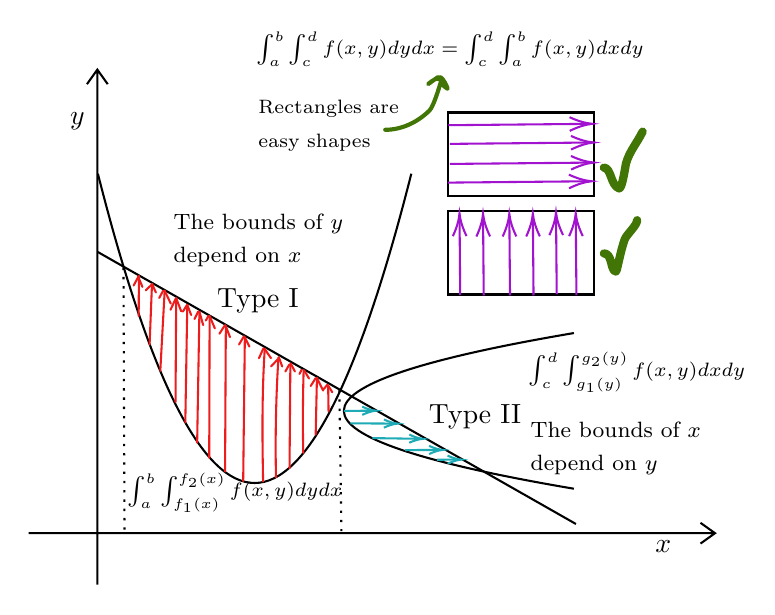
\begin{tikzpicture}[x=0.75pt,y=0.75pt,yscale=-1,xscale=1]
%uncomment if require: \path (0,300); %set diagram left start at 0, and has height of 300

%Shape: Axis 2D [id:dp15786148290852164] 
\draw  (66.67,256.35) -- (397.33,256.35)(99.73,33) -- (99.73,281.17) (390.33,251.35) -- (397.33,256.35) -- (390.33,261.35) (94.73,40) -- (99.73,33) -- (104.73,40)  ;
%Shape: Parabola [id:dp3374340259040851] 
\draw   (100,83.17) .. controls (150.33,281.83) and (200.67,281.83) .. (251,83.17) ;
%Straight Lines [id:da17471303708405084] 
\draw    (100,120.89) -- (330.33,251.92) ;
%Shape: Free Drawing [id:dp969312824964295] 
\draw  [color={rgb, 255:red, 237; green, 29; blue, 29 }  ,draw opacity=1 ][line width=0.75] [line join = round][line cap = round] (119.65,151.75) .. controls (119.68,145.3) and (119.72,138.84) .. (119.75,132.39) ;
%Shape: Free Drawing [id:dp25577323232811455] 
\draw  [color={rgb, 255:red, 237; green, 29; blue, 29 }  ,draw opacity=1 ][line width=0.75] [line join = round][line cap = round] (119.33,132.6) .. controls (120.04,134.28) and (120.74,135.96) .. (121.44,137.65) ;
%Shape: Free Drawing [id:dp5698702687630868] 
\draw  [color={rgb, 255:red, 237; green, 29; blue, 29 }  ,draw opacity=1 ][line width=0.75] [line join = round][line cap = round] (119.54,132.7) .. controls (118.77,134.14) and (118,135.58) .. (117.23,137.02) ;
%Shape: Free Drawing [id:dp29855586454232697] 
\draw  [color={rgb, 255:red, 237; green, 29; blue, 29 }  ,draw opacity=1 ][line width=0.75] [line join = round][line cap = round] (124.91,165.44) .. controls (125.3,155.68) and (125.68,145.93) .. (126.07,136.18) ;
%Shape: Free Drawing [id:dp5518305641486789] 
\draw  [color={rgb, 255:red, 237; green, 29; blue, 29 }  ,draw opacity=1 ][line width=0.75] [line join = round][line cap = round] (126.07,136.18) .. controls (126.7,137.58) and (127.33,138.98) .. (127.96,140.39) ;
%Shape: Free Drawing [id:dp3337563336556728] 
\draw  [color={rgb, 255:red, 237; green, 29; blue, 29 }  ,draw opacity=1 ][line width=0.75] [line join = round][line cap = round] (126.07,136.39) .. controls (125.09,137.37) and (124.11,138.35) .. (123.12,139.33) ;
%Shape: Free Drawing [id:dp7548434878361339] 
\draw  [color={rgb, 255:red, 237; green, 29; blue, 29 }  ,draw opacity=1 ][line width=0.75] [line join = round][line cap = round] (130.07,178.07) .. controls (130.77,165.23) and (131.47,152.39) .. (132.18,139.54) ;
%Shape: Free Drawing [id:dp3798761747267194] 
\draw  [color={rgb, 255:red, 237; green, 29; blue, 29 }  ,draw opacity=1 ][line width=0.75] [line join = round][line cap = round] (132.18,139.54) .. controls (133.16,141.61) and (134.14,143.68) .. (135.12,145.75) ;
%Shape: Free Drawing [id:dp032826386853152645] 
\draw  [color={rgb, 255:red, 237; green, 29; blue, 29 }  ,draw opacity=1 ][line width=0.75] [line join = round][line cap = round] (131.44,139.54) .. controls (130.81,140.7) and (130.18,141.86) .. (129.54,143.02) ;
%Shape: Free Drawing [id:dp03973270620885261] 
\draw  [color={rgb, 255:red, 237; green, 29; blue, 29 }  ,draw opacity=1 ][line width=0.75] [line join = round][line cap = round] (137.4,193.12) .. controls (137.51,176.39) and (137.61,159.65) .. (137.72,142.91) ;
%Shape: Free Drawing [id:dp5585733615581354] 
\draw  [color={rgb, 255:red, 237; green, 29; blue, 29 }  ,draw opacity=1 ][line width=0.75] [line join = round][line cap = round] (137.72,143.12) .. controls (138.53,145.23) and (139.33,147.33) .. (140.14,149.44) ;
%Shape: Free Drawing [id:dp09502119147890964] 
\draw  [color={rgb, 255:red, 237; green, 29; blue, 29 }  ,draw opacity=1 ][line width=0.75] [line join = round][line cap = round] (137.51,143.33) .. controls (136.67,145.12) and (135.82,146.91) .. (134.98,148.7) ;
%Shape: Free Drawing [id:dp5291512546852979] 
\draw  [color={rgb, 255:red, 237; green, 29; blue, 29 }  ,draw opacity=1 ][line width=0.75] [line join = round][line cap = round] (142.12,202.98) .. controls (142.43,184.12) and (142.75,165.25) .. (143.06,146.39) ;
%Shape: Free Drawing [id:dp5772349371864574] 
\draw  [color={rgb, 255:red, 237; green, 29; blue, 29 }  ,draw opacity=1 ][line width=0.75] [line join = round][line cap = round] (143.06,146.39) .. controls (143.69,148) and (144.31,149.61) .. (144.94,151.22) ;
%Shape: Free Drawing [id:dp1972925958236551] 
\draw  [color={rgb, 255:red, 237; green, 29; blue, 29 }  ,draw opacity=1 ][line width=0.75] [line join = round][line cap = round] (142.94,146.39) .. controls (142.27,147.45) and (141.61,148.51) .. (140.94,149.57) ;
%Shape: Free Drawing [id:dp8420460315730172] 
\draw  [color={rgb, 255:red, 237; green, 29; blue, 29 }  ,draw opacity=1 ][line width=0.75] [line join = round][line cap = round] (147.82,212.79) .. controls (148.18,191.76) and (148.55,170.73) .. (148.91,149.7) ;
%Shape: Free Drawing [id:dp27970958158007964] 
\draw  [color={rgb, 255:red, 237; green, 29; blue, 29 }  ,draw opacity=1 ][line width=0.75] [line join = round][line cap = round] (148.91,149.7) .. controls (149.52,151.82) and (150.12,153.94) .. (150.73,156.06) ;
%Shape: Free Drawing [id:dp5649824516326716] 
\draw  [color={rgb, 255:red, 237; green, 29; blue, 29 }  ,draw opacity=1 ][line width=0.75] [line join = round][line cap = round] (148.36,149.52) .. controls (147.76,150.73) and (147.15,151.94) .. (146.55,153.15) ;
%Shape: Free Drawing [id:dp3968145714534206] 
\draw  [color={rgb, 255:red, 237; green, 29; blue, 29 }  ,draw opacity=1 ][line width=0.75] [line join = round][line cap = round] (153.64,220.06) .. controls (153.7,197.27) and (153.76,174.48) .. (153.82,151.7) ;
%Shape: Free Drawing [id:dp6978169307097055] 
\draw  [color={rgb, 255:red, 237; green, 29; blue, 29 }  ,draw opacity=1 ][line width=0.75] [line join = round][line cap = round] (153.82,151.7) .. controls (154.67,153.7) and (155.52,155.7) .. (156.36,157.7) ;
%Shape: Free Drawing [id:dp8965668318145716] 
\draw  [color={rgb, 255:red, 237; green, 29; blue, 29 }  ,draw opacity=1 ][line width=0.75] [line join = round][line cap = round] (153.27,151.7) .. controls (152.85,152.42) and (152.42,153.15) .. (152,153.88) ;
%Shape: Free Drawing [id:dp973778437675962] 
\draw  [color={rgb, 255:red, 237; green, 29; blue, 29 }  ,draw opacity=1 ][line width=0.75] [line join = round][line cap = round] (161.27,226.61) .. controls (161.39,203.21) and (161.52,179.82) .. (161.64,156.42) ;
%Shape: Free Drawing [id:dp8382224187332488] 
\draw  [color={rgb, 255:red, 237; green, 29; blue, 29 }  ,draw opacity=1 ][line width=0.75] [line join = round][line cap = round] (161.64,156.61) .. controls (162.3,158.36) and (162.97,160.12) .. (163.64,161.88) ;
%Shape: Free Drawing [id:dp7905567713416519] 
\draw  [color={rgb, 255:red, 237; green, 29; blue, 29 }  ,draw opacity=1 ][line width=0.75] [line join = round][line cap = round] (161.27,156.06) .. controls (160.36,157.45) and (159.45,158.85) .. (158.55,160.24) ;
%Shape: Free Drawing [id:dp29787258326310195] 
\draw  [color={rgb, 255:red, 237; green, 29; blue, 29 }  ,draw opacity=1 ][line width=0.75] [line join = round][line cap = round] (170,231.23) .. controls (170.27,208.1) and (170.53,184.97) .. (170.8,161.83) ;
%Shape: Free Drawing [id:dp9274205944195231] 
\draw  [color={rgb, 255:red, 237; green, 29; blue, 29 }  ,draw opacity=1 ][line width=0.75] [line join = round][line cap = round] (170.8,162.03) .. controls (171.53,163.5) and (172.27,164.97) .. (173,166.43) ;
%Shape: Free Drawing [id:dp7693301223812206] 
\draw  [color={rgb, 255:red, 237; green, 29; blue, 29 }  ,draw opacity=1 ][line width=0.75] [line join = round][line cap = round] (170.4,161.43) .. controls (169.6,162.77) and (168.8,164.1) .. (168,165.43) ;
%Shape: Free Drawing [id:dp7782707170438627] 
\draw  [color={rgb, 255:red, 237; green, 29; blue, 29 }  ,draw opacity=1 ][line width=0.75] [line join = round][line cap = round] (179.6,231.43) .. controls (179.17,210.1) and (179.02,188.72) .. (180.4,167.43) ;
%Shape: Free Drawing [id:dp49133737965272806] 
\draw  [color={rgb, 255:red, 237; green, 29; blue, 29 }  ,draw opacity=1 ][line width=0.75] [line join = round][line cap = round] (180.4,167.63) .. controls (181.4,169.1) and (182.4,170.57) .. (183.4,172.03) ;
%Shape: Free Drawing [id:dp0785267232113096] 
\draw  [color={rgb, 255:red, 237; green, 29; blue, 29 }  ,draw opacity=1 ][line width=0.75] [line join = round][line cap = round] (179.8,167.23) .. controls (179.07,168.83) and (178.33,170.43) .. (177.6,172.03) ;
%Shape: Free Drawing [id:dp037346878597830147] 
\draw  [color={rgb, 255:red, 237; green, 29; blue, 29 }  ,draw opacity=1 ][line width=0.75] [line join = round][line cap = round] (185.8,229.43) .. controls (185.41,210.17) and (185.77,190.86) .. (187,171.63) ;
%Shape: Free Drawing [id:dp35237958666754987] 
\draw  [color={rgb, 255:red, 237; green, 29; blue, 29 }  ,draw opacity=1 ][line width=0.75] [line join = round][line cap = round] (187.2,171.63) .. controls (187.73,173.1) and (188.27,174.57) .. (188.8,176.03) ;
%Shape: Free Drawing [id:dp7470758145524414] 
\draw  [color={rgb, 255:red, 237; green, 29; blue, 29 }  ,draw opacity=1 ][line width=0.75] [line join = round][line cap = round] (186.8,172.43) .. controls (185.67,173.63) and (184.53,174.83) .. (183.4,176.03) ;
%Shape: Free Drawing [id:dp018728777026371768] 
\draw  [color={rgb, 255:red, 237; green, 29; blue, 29 }  ,draw opacity=1 ][line width=0.75] [line join = round][line cap = round] (192.33,225.03) .. controls (192.47,208.23) and (192.6,191.43) .. (192.73,174.63) ;
%Shape: Free Drawing [id:dp5653221017751002] 
\draw  [color={rgb, 255:red, 237; green, 29; blue, 29 }  ,draw opacity=1 ][line width=0.75] [line join = round][line cap = round] (192.93,174.63) .. controls (193.6,175.9) and (194.27,177.17) .. (194.93,178.43) ;
%Shape: Free Drawing [id:dp9541904640254413] 
\draw  [color={rgb, 255:red, 237; green, 29; blue, 29 }  ,draw opacity=1 ][line width=0.75] [line join = round][line cap = round] (192.13,175.23) .. controls (191.53,176.3) and (190.93,177.37) .. (190.33,178.43) ;
%Shape: Free Drawing [id:dp23599720315652117] 
\draw  [color={rgb, 255:red, 237; green, 29; blue, 29 }  ,draw opacity=1 ][line width=0.75] [line join = round][line cap = round] (198.93,217.63) .. controls (198.67,204.37) and (198.73,191.09) .. (199.13,177.83) ;
%Shape: Free Drawing [id:dp43705983027379713] 
\draw  [color={rgb, 255:red, 237; green, 29; blue, 29 }  ,draw opacity=1 ][line width=0.75] [line join = round][line cap = round] (199.33,177.83) .. controls (200.13,179.17) and (200.93,180.5) .. (201.73,181.83) ;
%Shape: Free Drawing [id:dp9423926335094328] 
\draw  [color={rgb, 255:red, 237; green, 29; blue, 29 }  ,draw opacity=1 ][line width=0.75] [line join = round][line cap = round] (198.13,177.63) .. controls (197.8,178.3) and (197.47,178.97) .. (197.13,179.63) ;
%Shape: Free Drawing [id:dp43649445090138905] 
\draw  [color={rgb, 255:red, 237; green, 29; blue, 29 }  ,draw opacity=1 ][line width=0.75] [line join = round][line cap = round] (204.93,208.83) .. controls (205.13,199.7) and (205.33,190.57) .. (205.53,181.43) ;
%Shape: Free Drawing [id:dp016088525454882152] 
\draw  [color={rgb, 255:red, 237; green, 29; blue, 29 }  ,draw opacity=1 ][line width=0.75] [line join = round][line cap = round] (205.53,181.63) .. controls (206.53,183.63) and (207.53,185.63) .. (208.53,187.63) ;
%Shape: Free Drawing [id:dp7012632769996316] 
\draw  [color={rgb, 255:red, 237; green, 29; blue, 29 }  ,draw opacity=1 ][line width=0.75] [line join = round][line cap = round] (204.93,181.63) .. controls (204.13,182.9) and (203.33,184.17) .. (202.53,185.43) ;
%Shape: Free Drawing [id:dp6952074944126365] 
\draw  [color={rgb, 255:red, 237; green, 29; blue, 29 }  ,draw opacity=1 ][line width=0.75] [line join = round][line cap = round] (211.13,197.63) .. controls (211.07,193.43) and (211,189.23) .. (210.93,185.03) ;
%Shape: Free Drawing [id:dp7366986048288056] 
\draw  [color={rgb, 255:red, 237; green, 29; blue, 29 }  ,draw opacity=1 ][line width=0.75] [line join = round][line cap = round] (210.93,185.23) .. controls (211.6,186.3) and (212.27,187.37) .. (212.93,188.43) ;
%Shape: Free Drawing [id:dp13202955261964755] 
\draw  [color={rgb, 255:red, 237; green, 29; blue, 29 }  ,draw opacity=1 ][line width=0.75] [line join = round][line cap = round] (210.53,184.83) .. controls (209.87,185.63) and (209.2,186.43) .. (208.53,187.23) ;
%Straight Lines [id:da45515719435402424] 
\draw  [dash pattern={on 0.84pt off 2.51pt}]  (112.33,128.42) -- (112.83,256.92) ;
%Straight Lines [id:da7085483760515869] 
\draw  [dash pattern={on 0.84pt off 2.51pt}]  (216.33,187.42) -- (217.33,255.33) ;
%Shape: Parabola [id:dp5275487206518001] 
\draw   (329.33,159.92) .. controls (181.55,184.92) and (181.55,209.92) .. (329.33,234.92) ;
%Straight Lines [id:da8367028978372462] 
\draw [color={rgb, 255:red, 30; green, 171; blue, 181 }  ,draw opacity=1 ]   (218.5,197.42) -- (231.93,197.34) ;
\draw [shift={(233.93,197.33)}, rotate = 179.69] [color={rgb, 255:red, 30; green, 171; blue, 181 }  ,draw opacity=1 ][line width=0.75]    (6.56,-1.97) .. controls (4.17,-0.84) and (1.99,-0.18) .. (0,0) .. controls (1.99,0.18) and (4.17,0.84) .. (6.56,1.97)   ;
%Straight Lines [id:da8809388553261903] 
\draw [color={rgb, 255:red, 30; green, 171; blue, 181 }  ,draw opacity=1 ]   (221.61,203.42) -- (242.37,203.54) ;
\draw [shift={(244.37,203.56)}, rotate = 180.35] [color={rgb, 255:red, 30; green, 171; blue, 181 }  ,draw opacity=1 ][line width=0.75]    (6.56,-1.97) .. controls (4.17,-0.84) and (1.99,-0.18) .. (0,0) .. controls (1.99,0.18) and (4.17,0.84) .. (6.56,1.97)   ;
%Straight Lines [id:da11309711757390795] 
\draw [color={rgb, 255:red, 30; green, 171; blue, 181 }  ,draw opacity=1 ]   (232.28,210.53) -- (254.59,210.86) ;
\draw [shift={(256.59,210.89)}, rotate = 180.85] [color={rgb, 255:red, 30; green, 171; blue, 181 }  ,draw opacity=1 ][line width=0.75]    (6.56,-1.97) .. controls (4.17,-0.84) and (1.99,-0.18) .. (0,0) .. controls (1.99,0.18) and (4.17,0.84) .. (6.56,1.97)   ;
%Straight Lines [id:da5582086187030633] 
\draw [color={rgb, 255:red, 30; green, 171; blue, 181 }  ,draw opacity=1 ]   (248.06,216.31) -- (264.15,216.23) ;
\draw [shift={(266.15,216.22)}, rotate = 179.74] [color={rgb, 255:red, 30; green, 171; blue, 181 }  ,draw opacity=1 ][line width=0.75]    (6.56,-1.97) .. controls (4.17,-0.84) and (1.99,-0.18) .. (0,0) .. controls (1.99,0.18) and (4.17,0.84) .. (6.56,1.97)   ;
%Straight Lines [id:da7346180773807092] 
\draw [color={rgb, 255:red, 30; green, 171; blue, 181 }  ,draw opacity=1 ]   (263.39,220.97) -- (273.04,220.9) ;
\draw [shift={(275.04,220.89)}, rotate = 179.59] [color={rgb, 255:red, 30; green, 171; blue, 181 }  ,draw opacity=1 ][line width=0.75]    (6.56,-1.97) .. controls (4.17,-0.84) and (1.99,-0.18) .. (0,0) .. controls (1.99,0.18) and (4.17,0.84) .. (6.56,1.97)   ;
%Shape: Rectangle [id:dp9480019119606491] 
\draw   (268.89,53.67) -- (338.89,53.67) -- (338.89,93.67) -- (268.89,93.67) -- cycle ;
%Straight Lines [id:da45246609161389517] 
\draw [color={rgb, 255:red, 161; green, 19; blue, 207 }  ,draw opacity=1 ]   (268.89,59.78) -- (336.22,59.13) ;
\draw [shift={(338.22,59.11)}, rotate = 179.45] [color={rgb, 255:red, 161; green, 19; blue, 207 }  ,draw opacity=1 ][line width=0.75]    (10.93,-3.29) .. controls (6.95,-1.4) and (3.31,-0.3) .. (0,0) .. controls (3.31,0.3) and (6.95,1.4) .. (10.93,3.29)   ;
%Straight Lines [id:da06974333669582844] 
\draw [color={rgb, 255:red, 161; green, 19; blue, 207 }  ,draw opacity=1 ]   (269.56,68.78) -- (336.89,68.13) ;
\draw [shift={(338.89,68.11)}, rotate = 179.45] [color={rgb, 255:red, 161; green, 19; blue, 207 }  ,draw opacity=1 ][line width=0.75]    (10.93,-3.29) .. controls (6.95,-1.4) and (3.31,-0.3) .. (0,0) .. controls (3.31,0.3) and (6.95,1.4) .. (10.93,3.29)   ;
%Straight Lines [id:da4041509235794307] 
\draw [color={rgb, 255:red, 161; green, 19; blue, 207 }  ,draw opacity=1 ]   (269.56,78.44) -- (336.89,77.8) ;
\draw [shift={(338.89,77.78)}, rotate = 179.45] [color={rgb, 255:red, 161; green, 19; blue, 207 }  ,draw opacity=1 ][line width=0.75]    (10.93,-3.29) .. controls (6.95,-1.4) and (3.31,-0.3) .. (0,0) .. controls (3.31,0.3) and (6.95,1.4) .. (10.93,3.29)   ;
%Straight Lines [id:da7624228898208436] 
\draw [color={rgb, 255:red, 161; green, 19; blue, 207 }  ,draw opacity=1 ]   (268.56,87.44) -- (335.89,86.8) ;
\draw [shift={(337.89,86.78)}, rotate = 179.45] [color={rgb, 255:red, 161; green, 19; blue, 207 }  ,draw opacity=1 ][line width=0.75]    (10.93,-3.29) .. controls (6.95,-1.4) and (3.31,-0.3) .. (0,0) .. controls (3.31,0.3) and (6.95,1.4) .. (10.93,3.29)   ;
%Shape: Rectangle [id:dp601771782879176] 
\draw   (268.89,101.33) -- (338.89,101.33) -- (338.89,141.33) -- (268.89,141.33) -- cycle ;
%Straight Lines [id:da8378667824988064] 
\draw [color={rgb, 255:red, 161; green, 19; blue, 207 }  ,draw opacity=1 ]   (274.56,141.61) -- (274.24,104.28) ;
\draw [shift={(274.22,102.28)}, rotate = 89.51] [color={rgb, 255:red, 161; green, 19; blue, 207 }  ,draw opacity=1 ][line width=0.75]    (10.93,-3.29) .. controls (6.95,-1.4) and (3.31,-0.3) .. (0,0) .. controls (3.31,0.3) and (6.95,1.4) .. (10.93,3.29)   ;
%Straight Lines [id:da9054730509858795] 
\draw [color={rgb, 255:red, 161; green, 19; blue, 207 }  ,draw opacity=1 ]   (285.89,141.78) -- (285.57,104.44) ;
\draw [shift={(285.56,102.44)}, rotate = 89.51] [color={rgb, 255:red, 161; green, 19; blue, 207 }  ,draw opacity=1 ][line width=0.75]    (10.93,-3.29) .. controls (6.95,-1.4) and (3.31,-0.3) .. (0,0) .. controls (3.31,0.3) and (6.95,1.4) .. (10.93,3.29)   ;
%Straight Lines [id:da11283440285410418] 
\draw [color={rgb, 255:red, 161; green, 19; blue, 207 }  ,draw opacity=1 ]   (298.56,141.78) -- (298.24,104.44) ;
\draw [shift={(298.22,102.44)}, rotate = 89.51] [color={rgb, 255:red, 161; green, 19; blue, 207 }  ,draw opacity=1 ][line width=0.75]    (10.93,-3.29) .. controls (6.95,-1.4) and (3.31,-0.3) .. (0,0) .. controls (3.31,0.3) and (6.95,1.4) .. (10.93,3.29)   ;
%Straight Lines [id:da9892820301431604] 
\draw [color={rgb, 255:red, 161; green, 19; blue, 207 }  ,draw opacity=1 ]   (309.89,141.78) -- (309.57,104.44) ;
\draw [shift={(309.56,102.44)}, rotate = 89.51] [color={rgb, 255:red, 161; green, 19; blue, 207 }  ,draw opacity=1 ][line width=0.75]    (10.93,-3.29) .. controls (6.95,-1.4) and (3.31,-0.3) .. (0,0) .. controls (3.31,0.3) and (6.95,1.4) .. (10.93,3.29)   ;
%Straight Lines [id:da2461511880160343] 
\draw [color={rgb, 255:red, 161; green, 19; blue, 207 }  ,draw opacity=1 ]   (321.06,141.11) -- (320.74,103.78) ;
\draw [shift={(320.72,101.78)}, rotate = 89.51] [color={rgb, 255:red, 161; green, 19; blue, 207 }  ,draw opacity=1 ][line width=0.75]    (10.93,-3.29) .. controls (6.95,-1.4) and (3.31,-0.3) .. (0,0) .. controls (3.31,0.3) and (6.95,1.4) .. (10.93,3.29)   ;
%Straight Lines [id:da7863932760583598] 
\draw [color={rgb, 255:red, 161; green, 19; blue, 207 }  ,draw opacity=1 ]   (330.56,141.61) -- (330.24,104.28) ;
\draw [shift={(330.22,102.28)}, rotate = 89.51] [color={rgb, 255:red, 161; green, 19; blue, 207 }  ,draw opacity=1 ][line width=0.75]    (10.93,-3.29) .. controls (6.95,-1.4) and (3.31,-0.3) .. (0,0) .. controls (3.31,0.3) and (6.95,1.4) .. (10.93,3.29)   ;
%Shape: Free Drawing [id:dp5778331674629196] 
\draw  [color={rgb, 255:red, 65; green, 117; blue, 5 }  ,draw opacity=1 ][line width=3] [line join = round][line cap = round] (362.44,62.89) .. controls (359.41,68.95) and (356.18,72.16) .. (354.44,78.22) .. controls (354.17,79.17) and (352.59,90.71) .. (351.11,90.22) .. controls (347.02,88.86) and (347.32,80.22) .. (343.78,80.22) ;
%Shape: Free Drawing [id:dp9367905772564737] 
\draw  [color={rgb, 255:red, 65; green, 117; blue, 5 }  ,draw opacity=1 ][line width=3] [line join = round][line cap = round] (359.78,105.56) .. controls (359.78,108.17) and (354.67,112.34) .. (353.78,114.89) .. controls (352.34,119.01) and (351.46,123.31) .. (350.44,127.56) .. controls (350.21,128.52) and (349.91,130.82) .. (349.11,130.22) .. controls (346.82,128.5) and (347.74,121.56) .. (343.78,121.56) ;
%Shape: Free Drawing [id:dp6361197696653147] 
\draw  [color={rgb, 255:red, 65; green, 117; blue, 5 }  ,draw opacity=1 ][line width=1.5] [line join = round][line cap = round] (238.44,62) .. controls (246.47,62) and (254.2,58.24) .. (259.78,52.67) .. controls (261.73,50.72) and (264.35,41.79) .. (265.11,39.33) .. controls (265.37,38.48) and (264.42,36.11) .. (265.11,36.67) .. controls (266.75,37.98) and (267.71,40.04) .. (268.44,42) .. controls (268.73,42.75) and (267.11,41.11) .. (266.44,40.67) .. controls (265.37,39.95) and (265.67,37.74) .. (264.44,37.33) .. controls (262.56,36.7) and (259.11,40) .. (259.11,40) .. controls (259.11,40) and (263.36,36.87) .. (263.78,36.67) ;

% Text Node
\draw (156,137) node [anchor=north west][inner sep=0.75pt]   [align=left] {Type I};
% Text Node
\draw (258,193) node [anchor=north west][inner sep=0.75pt]   [align=left] {Type II};
% Text Node
\draw (134.99,101.12) node [anchor=north west][inner sep=0.75pt]  [rotate=-359.93] [align=left] {{\footnotesize The bounds of $\displaystyle y$}\\{\footnotesize depend on $\displaystyle x$}};
% Text Node
\draw (306.99,201.46) node [anchor=north west][inner sep=0.75pt]  [rotate=-359.93] [align=left] {{\footnotesize The bounds of $\displaystyle x$}\\{\footnotesize depend on $\displaystyle y$}};
% Text Node
\draw (175.83,46.33) node [anchor=north west][inner sep=0.75pt]   [align=left] {{\scriptsize Rectangles are}\\{\scriptsize easy shapes}};
% Text Node
\draw (174.83,13.29) node [anchor=north west][inner sep=0.75pt]  [font=\scriptsize]  {$\int _{a}^{b}\int _{c}^{d} f(x,y)dydx=\int _{c}^{d}\int _{a}^{b} f(x,y)dxdy$};
% Text Node
\draw (112.83,225.73) node [anchor=north west][inner sep=0.75pt]  [font=\scriptsize]  {$\int _{a}^{b}\int _{f_{1}( x)}^{f_{2}( x)} f(x,y)dydx$};
% Text Node
\draw (306.16,167.73) node [anchor=north west][inner sep=0.75pt]  [font=\scriptsize]  {$\int _{c}^{d}\int _{g_{1}( y)}^{g_{2}( y)} f(x,y)dxdy$};
% Text Node
\draw (367.11,258.4) node [anchor=north west][inner sep=0.75pt]    {$x$};
% Text Node
\draw (85.11,52.4) node [anchor=north west][inner sep=0.75pt]    {$y$};


\end{tikzpicture}

\fi


\end{frame}

\begin{frame}{General regions}
    %The question is often: ``find the volume of the solid body between the xy-plane and the function $f(x,y)$ which is above the \textit{region .....}"

    %This ``region" is then the region we're integrating over. Very often, these regions are \textbf{general regions}, which can be either type I or type II.
    \begin{theorybox}{Double integrals over general regions}
    A type I region goes like this:
    \[D=\{(x,y)\mid a\leq x\leq b,~ g_1(x)\leq y\leq g_2(x)\}\]
        \[\iint_D f(x,y)dA=\int_a^b\int_{g_1(x)}^{g_2(x)}f(x,y)dydx\]

    \pause A type II region goes like this:
    \[D=\{(x,y)\mid c\leq y\leq d,~ h_1(y)\leq x\leq h_2(y)\}\]
        \[\iint_D f(x,y)dA=\int_c^d\int_{h_1(y)}^{h_2(y)}f(x,y)dxdy\]
    \end{theorybox}
\end{frame}

\begin{frame}{Double integrals over general regions (1/2)}
         \textbf{Question:} calculate the volume of the 3D body between the paraboloid $z=x^2+y^2$ and the $xy$-plane, above the region $D$ enclosed by the parabola $y=3x^2$ and the line $y=x+2$.

            \begin{minipage}{0.38\textwidth}
\begin{tikzpicture}
\begin{axis}[
    xlabel = \(x\),
    ylabel = {\(y\)},
    axis lines=middle,
    height=6cm,
    width=7cm,
]
\addplot [
    domain=-2:2, 
    samples=100, 
    color=red,
    name path=f,
]
{3*x^2};
    \addlegendentry{\(3x^2\)}
\addplot [
    domain=-2:2, 
    samples=100, 
    color=blue,
    name path=g,
    ]
    {x+2};
    \addlegendentry{\(x+2\)}

    \addplot[teal!10, opacity=0.9] fill between[of=f and g, soft clip={domain=-0.667:1}];
\node at (axis cs:0.2,1.2) {$D$};
\end{axis}
\end{tikzpicture}
            \end{minipage}\hspace{1.5cm}
            \begin{minipage}{0.47\textwidth}

                \pause Solving the equation $3x^2=x+2$ gives the endpoints $x=-\frac{2}{3}$ and $x=1$, so we get a type I\footnote{The region of integration $D=\{(x,y)\mid-\frac{2}{3}\leq x\leq1,~3x^2\leq y\leq x+2\}$} \vspace{-2mm}\[V=\iint_{D}(x^2+y^2)dA\]\vspace{-2mm}\[\boxed{V=\int_{-2/3}^{1}\int_{3x^2}^{x+2}(x^2+y^2)dydx}\]
To be computed in the next slide.
            \end{minipage}

\end{frame}

\begin{frame}{Double integrals over general regions (2/2)}
\small
         We calculate the integral from the previous slide to find the volume:
         \begin{align*}
             V&=\int_{-2/3}^{1}\int_{3x^2}^{x+2}(x^2+y^2)dydx=\int_{-2/3}^{1}\left[x^2y+\frac{y^3}{3}\right]_{y=3x^2}^{y=x+2}dx\\
              &=\int_{-2/3}^{1}\left[x^2(x+2)+\frac{1}{3}(x+2)^3-x^2\cdot3x^2-\frac{1}{3}(3x^2)^3\right]dx\\
              &=\int_{-2/3}^{1}\left[x^3+2x^2+\frac{1}{3}\left(x^3+6x^2+12x+8\right)-3x^4-9x^6\right]dx\\
              &=\int_{-2/3}^{1}\left(-9x^6-3x^4+\frac{4}{3}x^3+4x^2+4x+\frac{8}{3}\right)dx\\
              &=\left[-\frac{9}{7}x^7-\frac{3}{5}x^5+\frac{1}{3}x^4+\frac{4}{3}x^3+2x^2+\frac{8}{3}x\right]_{-2/3}^{1} =\boxed{ \frac{3125}{567}}
         \end{align*}
         \pause So the volume is $\frac{3125}{567}$. \textbf{Note:} in this case, the order of integration matters. We have to first integrate w.r.t. $y$ and then $x$. (Try the other way, it's very hard.)
\end{frame}

\begin{frame}{Order of integration can matter}
    \small
    \begin{itemize}
        \item \textbf{Question:} evaluate $\iint_De^{y^2}dA$, where the region of integration is
            $D=\{(x,y)\mid 0\leq x\leq1,~5x\leq y\leq5\}$
        \item\pause \textbf{Step $\pmb{-\infty}$:} write a Type I integral:
            \[\iint_De^{y^2}dA=\int_0^1\int_{5x}^5e^{y^2}dydx\]
        \pause Observe that we have a problem: we can't find the antiderivative of $e^{y^2}$.
        \item\pause \textbf{Step 1:} rewrite the region as\footnote{To see this, draw out the (triangular) region on paper}
            $D=\left\{(x,y)\mid 0\leq y\leq5,~0\leq x\leq\frac{y}{5}\right\}$
        \item\pause \textbf{Step 2:} write a Type II integral and solve it:
            \begin{align*}
                \iint_D&e^{y^2}dA=\int_0^5\int_0^{y/5}e^{y^2}dxdy = \int_0^5 \left[xe^{y^2}\right]_{x=0}^{x=y/5}dy=\frac{1}{5}\int_0^5ye^{y^2}dy\\
                &=\frac{1}{5}\left[\frac{1}{2}e^{y^2}\right]_0^5=\boxed{\frac{1}{10}(e^{25}-1)}
            \end{align*}
    \end{itemize}
\end{frame}

\subsection{In polar coordinates ($r,\theta$)}
\tableofcontents[currentsection,currentsubsection]
\begin{frame}{Polar coordinates (1/2)}
    Sometimes we need to do integrals using \textbf{polar coordinates}. The polar coordinate system uses $r$ for radial distance and $\theta$ is the angular coordinate. The polar system looks like this:

    \vspace{0.3mm}
    \begin{minipage}{0.6\textwidth}
    \tikzset{every picture/.style={line width=0.75pt}} %set default line width to 0.75pt        

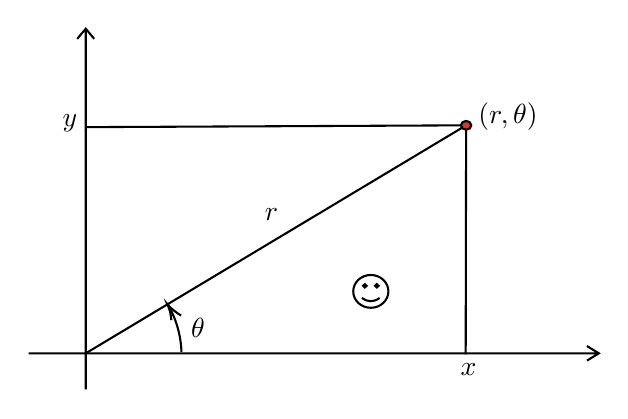
\begin{tikzpicture}[x=0.75pt,y=0.75pt,yscale=-0.7,xscale=0.82]
%uncomment if require: \path (0,285); %set diagram left start at 0, and has height of 285

%Shape: Smiley Face [id:dp830203050540306] 
\draw   (201.67,196.79) .. controls (201.67,190.56) and (206.29,185.5) .. (212,185.5) .. controls (217.71,185.5) and (222.33,190.56) .. (222.33,196.79) .. controls (222.33,203.03) and (217.71,208.08) .. (212,208.08) .. controls (206.29,208.08) and (201.67,203.03) .. (201.67,196.79) -- cycle ; \draw   (207.45,192.95) .. controls (207.45,192.33) and (207.92,191.82) .. (208.49,191.82) .. controls (209.06,191.82) and (209.52,192.33) .. (209.52,192.95) .. controls (209.52,193.58) and (209.06,194.08) .. (208.49,194.08) .. controls (207.92,194.08) and (207.45,193.58) .. (207.45,192.95) -- cycle ; \draw   (214.48,192.95) .. controls (214.48,192.33) and (214.94,191.82) .. (215.51,191.82) .. controls (216.08,191.82) and (216.55,192.33) .. (216.55,192.95) .. controls (216.55,193.58) and (216.08,194.08) .. (215.51,194.08) .. controls (214.94,194.08) and (214.48,193.58) .. (214.48,192.95) -- cycle ; \draw   (206.83,201.31) .. controls (210.28,204.32) and (213.72,204.32) .. (217.17,201.31) ;
%Shape: Axis 2D [id:dp26103124522186905] 
\draw  (11,239.43) -- (346,239.43)(44.5,16) -- (44.5,264.25) (339,234.43) -- (346,239.43) -- (339,244.43) (39.5,23) -- (44.5,16) -- (49.5,23)  ;
%Straight Lines [id:da3997877631677582] 
\draw    (268,82.5) -- (267.75,240.13) ;
%Straight Lines [id:da143433628895133] 
\draw    (268,82.5) -- (44.5,239.43) ;
%Curve Lines [id:da0981281691186493] 
\draw    (100.71,238.5) .. controls (100.71,233.28) and (99.44,218.76) .. (92.82,206.27) ;
\draw [shift={(92.38,205.46)}, rotate = 61.07] [color={rgb, 255:red, 0; green, 0; blue, 0 }  ][line width=0.75]    (10.93,-3.29) .. controls (6.95,-1.4) and (3.31,-0.3) .. (0,0) .. controls (3.31,0.3) and (6.95,1.4) .. (10.93,3.29)   ;
%Straight Lines [id:da7865700687572084] 
\draw    (268,82.5) -- (44.67,83.75) ;
%Shape: Circle [id:dp17179590489530172] 
\draw  [fill={rgb, 255:red, 229; green, 47; blue, 47 }  ,fill opacity=1 ] (264.96,82.5) .. controls (264.96,80.82) and (266.32,79.46) .. (268,79.46) .. controls (269.68,79.46) and (271.04,80.82) .. (271.04,82.5) .. controls (271.04,84.18) and (269.68,85.54) .. (268,85.54) .. controls (266.32,85.54) and (264.96,84.18) .. (264.96,82.5) -- cycle ;

% Text Node
\draw (263,244.65) node [anchor=north west][inner sep=0.75pt]    {$x$};
% Text Node
\draw (29.17,72.65) node [anchor=north west][inner sep=0.75pt]    {$y$};
% Text Node
\draw (104.67,212.98) node [anchor=north west][inner sep=0.75pt]    {$\theta $};
% Text Node
\draw (148,137.65) node [anchor=north west][inner sep=0.75pt]    {$r$};
% Text Node
\draw (273.33,64.98) node [anchor=north west][inner sep=0.75pt]    {$( r,\theta )$};


\end{tikzpicture}

    \end{minipage}
    \begin{minipage}{0.35\textwidth}
        We see the important equations for polar coordinates, which we use a lot:
        \[\boxed{x^2+y^2=r^2}\]
        \[\boxed{x=r\cos\theta}\]
        \[\boxed{y=r\sin\theta}\]
    \end{minipage}
\end{frame}

\begin{frame}{Polar coordinates (2/2)}
    Back in normal coordinates, we could just say $dA=dx\,dy$ (or $dA=dy\,dx$). For example:
    \[D=\{(x,y)~\mid~y\leq x\leq y+2~\land~1\leq y\leq 3\}\]
    \[\iint_D f(x,y) \red{dA} = \int_{1}^{3}\int_{y}^{y+2}f(x,y)\red{dx\,dy}\]

    \pause For polar regions, we replace $dA$ with $r\cdot dr\,d\theta$ (or $r\cdot d\theta\, dr$). For example:
    \[D=\{(r,\theta)~\mid~1\leq r\leq 2~\land~0\leq\theta\leq2\pi\}\]
    \[\iint_D f(r,\theta) \red{dA} = \int_{0}^{2\pi}\int_{1}^{2}f(r,\theta)\red{r\,dr\,d\theta}\]
    \red{\textbf{IMPORTANT: it is $dA=r\cdot dr\,d\theta$, NOT $dA=dr\,d\theta$.}} (This factor $r$ is the ``Jacobian", do not forget to write it when doing polar coordinates!)
\end{frame}


\begin{frame}{A ``polar" integral}
\footnotesize
    \begin{itemize}
        \item \textbf{Question:} calculate the volume of the solid body bounded by the function $z=f(x,y)=x^4+2x^2y^2+y^4$ and the $xy$-plane above the circular region in the $xy$-plane given in the plot:

            \begin{minipage}{0.35\textwidth}
\begin{tikzpicture}
\begin{axis}[
    xlabel = \(x\),
    ylabel = {\(y\)},
    axis lines=middle,
    height=5cm,
    width=4.7cm,
    xmin=-0.6,xmax=2.5,
    ymin=-2.5,ymax=2.5,
    ytick distance=1,
]
\addplot [
    domain=-1:3.5, 
    samples=300, 
    color=red,
    name path=f,
]
    {sqrt(1-x^2)};
\addplot [
    domain=-1:3, 
    samples=300, 
    color=blue,
    name path=h,
]
    {sqrt(4-x^2)};
\addplot [
    domain=-1:3.5, 
    samples=300, 
    color=red,
    name path=g,
    ]
    {-sqrt(1-x^2)};
\addplot [
    domain=-1:2.5, 
    samples=300, 
    color=blue,
    name path=i,
    ]
    {-sqrt(4-x^2)};

\node at (axis cs:1.7,0.2) {$D$};
    \addplot[teal!10, opacity=0.9] fill between[of=f and h, soft clip={domain=0:1.1}];
    \addplot[teal!10, opacity=0.9] fill between[of=h and i, soft clip={domain=1:3}];
    \addplot[teal!10, opacity=0.9] fill between[of=g and i, soft clip={domain=0:1.1}];
\end{axis}
\end{tikzpicture}
            \end{minipage}\begin{minipage}{0.6\textwidth}
                    \item\pause \textbf{Step 1:} we can write the region of the plot as
                        \[D=\{(r,\theta)~\mid~ 1\leq r\leq2 ~\land~ -\pi/2\leq\theta\leq\pi/2\}\]
                    \item\pause \textbf{Step 2:} we have \[f(x,y)=x^4+2x^2y^2+y^4=(x^2+y^2)^2\] Using the identity $x^2+y^2=r^2$, we see that this is equal to $(r^2)^2=r^4$.
            \end{minipage}
        \item\pause \textbf{Step 3:} set up the integral and solve it (don't forget the extra factor $\blue{r}$ due to polar coordinates):
            \[V=\int_{-\pi/2}^{\pi/2}\int_1^2 r^4 \blue{r}\,dr\,d\theta=\int_{-\pi/2}^{\pi/2}d\theta\int_1^2 r^5 dr=\pi\left[\frac{1}{6}r^6\right]_1^2=\boxed{\frac{21}{2}\pi}\]
                        So the volume is $\frac{21}{2}\pi$.
    \end{itemize}
\end{frame}

%\begin{frame}{Nasty little question}
%\footnotesize
%    \begin{itemize}
%        \item \textbf{Question:} calculate the volume of the solid body bounded by the function $z=f(x,y)=y\sqrt{x^2+y^2}$ and the $xy$-plane above the shaded region in the $xy$-plane given in the plot (note: only consider $y\geq0$):
%
%            \begin{minipage}{0.45\textwidth}
%\begin{tikzpicture}
%\begin{axis}[
%    xlabel = \(x\),
%    ylabel = {\(y\)},
%    axis lines=middle,
%    height=5cm,
%    width=6.4cm,
%    xmin=-3,ymin=-3,
%    xmax=7,ymax=4,
%]
%    \addplot[domain=0:pi,samples=100,color=red,data cs=polarrad, name path = f] { 3+2*cos(deg(x))};
%    \addplot[domain=0:pi,samples=100,color=violet,data cs=polarrad,name path=g] { 2};
%    \addplot[teal!10, opacity=0.9] fill between[of=g and f, split];
%
%\node at (axis cs:2.8,1.8) {$D$};
%\end{axis}
%\end{tikzpicture}
%            \end{minipage}\begin{minipage}{0.45\textwidth}
%                Here, it is given that the red border is described by the equation \[\sqrt{x^2+y^2}=3+\frac{2x}{\sqrt{x^2+y^2}}\] And the violet border is described by the equation \[x^2+y^2=4\]
%            \end{minipage}
%        \item \textbf{Solution:} next slide
%    \end{itemize}
%\end{frame}


\begin{frame}{A harder polar integral (1/4)}
\footnotesize
    \begin{itemize}
        \item \textbf{Question:} calculate the volume of the solid body bounded by the function $z=f(x,y)=y\sqrt{x^2+y^2}$ and the $xy$-plane above the shaded region in the $xy$-plane given in the plot (note: only consider $y\geq0$):

\begin{tikzpicture}
\begin{axis}[
    xlabel = \(x\),
    ylabel = {\(y\)},
    axis lines=middle,
    height=5cm,
    width=6.4cm,
    xmin=-3,ymin=-3,
    xmax=7,ymax=4,
    legend pos=outer north east,
    legend style={minimum height=7mm}
]
    \addplot[domain=0:pi,samples=100,color=red,data cs=polarrad, name path=f] { 3+2*cos(deg(x))};
    \addlegendentry{\(\sqrt{x^2+y^2}=3+\frac{2x}{\sqrt{x^2+y^2}}\)}
    \addplot[domain=0:pi,samples=100,color=blue,data cs=polarrad,name path=g] { 2};
    \addlegendentry{\({x^2+y^2}=4\)}
    \addplot[domain=0:pi,samples=100,color=teal,data cs=polarrad,name path=h] { 1};
    \addlegendentry{\({x^2+y^2}=1\)}
    \addplot[teal!17, opacity=0.9] fill between[of=g and f, split];
    \addplot[teal!17, opacity=0.9] fill between[of=g and h];

\node at (axis cs:1.9,1.6) {$D$};
\end{axis}
\end{tikzpicture}
        \item \textbf{Solution:} next slide
    \end{itemize}
\end{frame}


\begin{frame}{A harder polar integral (2/4)}
    \begin{itemize}
        \item Let's first rewrite the equation of the red boundary into polar coordinates (use $x^2+y^2=r^2$ and $x=r\cos\theta$):
            \[\sqrt{x^2+y^2}=3+\frac{2x}{\sqrt{x^2+y^2}} \quad\red{\rightsquigarrow}\quad \pmb{\red{r=3+2\cos\theta}}\]
        \item\pause The other boundaries are just half-circles with radii $r=1$ and $\pmb{\blue{r=2}}$.
    \end{itemize}

    \vspace{3mm}
\begin{minipage}{0.45\textwidth}
\begin{tikzpicture}
\begin{axis}[
    xlabel = \(x\),
    ylabel = {\(y\)},
    axis lines=middle,
    height=5cm,
    width=6.4cm,
    xmin=-3,ymin=-3,
    xmax=7,ymax=4,
    legend pos=outer north east,
    legend style={minimum height=7mm},
   % every axis plot/.append style={ultra thick}
]
    \addplot[domain=0:pi,samples=100,color=red,data cs=polarrad, name path=f, style={ultra thick}] { 3+2*cos(deg(x))};
    \addplot[domain=0:pi,samples=300,color=blue,data cs=polarrad,name path=g, style={ultra thick}] { 2};
    \addplot[domain=0:pi,samples=300,color=teal,data cs=polarrad,name path=h] { 1};
    \addplot[domain=-2:7,samples=300,draw=none,name path=j] { 0};
    \addplot[domain=-1:0,samples=300,color=blue,name path=i] {-sqrt(3)*x};
    \addplot[magenta!17, opacity=0.9] fill between[of=h and f,
    soft clip=i
    ];
    \addplot[orange, opacity=0.9] fill between[of=g and j,soft clip={domain=-2:-1}];
    \addplot[orange, opacity=0.9] fill between[of=h and i,soft clip={domain=-1:-0.5}];

\node at (axis cs:2.6,1.6) {$D_1$};
\node at (axis cs:-1.4,0.7) {$D_2$};
    \coordinate (aaa) at (axis cs:3,0);
    \coordinate (bbb) at (axis cs:0,0);
    \coordinate (ccc) at (axis cs:-1,1.732);
    \pic [draw, ->, "$\theta$", angle eccentricity=2.17, angle radius=1.4mm] {angle = aaa--bbb--ccc};
\end{axis}
\end{tikzpicture}
%\begin{tikzpicture}
%\begin{axis}[
%    xlabel = \(x\),
%    ylabel = {\(y\)},
%    axis lines=middle,
%    height=5cm,
%    width=6.4cm,
%    xmin=-3,ymin=-3,
%    xmax=7,ymax=4,
%]
%    \addplot[domain=0:pi,samples=100,color=red,data cs=polarrad, name path = f] { 3+2*cos(deg(x))};
%    \addplot[domain=0:pi,samples=100,color=violet,data cs=polarrad,name path=g] { 2};
%    \addplot[yellow, opacity=0.9] fill between[of=g and f, split, every odd segment/.style={gray}];
%
%\end{axis}
%\end{tikzpicture}
            \end{minipage}\begin{minipage}{0.45\textwidth}
                \pause We need to split the region; see the picture.\footnote{There are also other ways to split} The angle $\theta$ as in the picture occurs when $\blue{r_{\text{blue}}}=\red{r_{\text{red}}}$ \[\pmb{\blue{2}=\red{3+2\cos\theta}}\quad\Rightarrow\quad\cos\theta=-\frac{1}{2}\]
                \pause So we split the integral at $\theta=\frac{2}{3}\pi$.
                
            \end{minipage}
\end{frame}




\begin{frame}{A harder polar integral (3/4)}
    \footnotesize
                In the previous slide, we calculated that the ``split angle'' is $\theta=\frac{2\pi}{3}$.  

            \pause We can write the region of integration as $D=D_1\cup D_2$ (with $D_{1,2}$ as in the picture on previous slide, note that these regions do not overlap except at the boundary):
            \begin{align*}D &=\{(r,\theta) \mid 0\leq\theta\leq\frac{2\pi}{3} \land 1\leq r\leq 3+2\cos\theta \}\\&\qquad\cup\{(r,\theta) \mid \frac{2\pi}{3}\leq\theta\leq\pi \land 1\leq r\leq2\}\end{align*}

                \pause We obtain (since $z=\red{f(x,y)}=y\sqrt{x^2+y^2}=(r\sin\theta)r=\red{r^2\sin\theta}$) \begin{align*}V&=\iint_{D}\red{f(x,y)}\blue{dA}=\iint_{D_1}\red{f(x,y)}\blue{dA}+\iint_{D_2}\red{f(x,y)}\blue{dA}\\&=\int_0^{2\pi/3}\int_1^{3+2\cos\theta}\red{(r^2\sin\theta)}\blue{r\,dr\,d\theta}+\int_{2\pi/3}^{\pi}\int_{1}^2\red{(r^2\sin\theta)} \blue{r\,dr\,d\theta}\end{align*}
            To be computed in the next slide.

\end{frame}

\begin{frame}{A harder polar integral (4/4)}
    \footnotesize
    \begin{align*}
        \onslide<1->{V&=\int_0^{2\pi/3}\int_1^{3+2\cos\theta}(r^2\sin\theta)r\,dr\,d\theta+\int_{2\pi/3}^{\pi}\int_{1}^2(r^2\sin\theta) r\,dr\,d\theta\\[-1mm]}
         \onslide<2->{&\qquad\yellow{\text{\scriptsize ($*$ Rewrite integral, see next slide for detailed explanation $*$)}}\\[-1mm]
         &=\int_0^{2\pi/3}\sin\theta\int_1^{3+2\cos\theta}r^3dr\,d\theta+\int_{2\pi/3}^{\pi}\sin\theta d\theta\int_{1}^2r^3 dr\\[-1mm]}
         \onslide<3->{&=\int_0^{2\pi/3}\sin\theta\left[\frac{r^4}{4}\right]_1^{3+2\cos\theta}d\theta+\left(\left[-\cos\theta\right]_{2\pi/3}^{\pi} \left[\frac{r^4}{4}\right]_1^2\right)\\[-1mm]}
         \onslide<4->{&=\frac{1}{4}\int_0^{2\pi/3}\sin\theta\left((3+2\cos\theta)^4-1\right)d\theta+\left(\left[-\cos\theta\right]_{2\pi/3}^{\pi} \left[\frac{r^4}{4}\right]_1^2\right)\\[-1mm]}
         \onslide<5->{&\qquad\yellow{\text{\scriptsize ($*$ Antiderivative of $(\sin\theta)(3+2\cos\theta)^4$ can be found by subbing $u=3+2\cos\theta$ $*$)}}\\[-1mm]
         &=\frac{1}{4}\left[-\frac{1}{10}(3+2\cos\theta)^5+\cos\theta\right]_0^{2\pi/3}+\frac{15}{8}=\frac{1}{4}\left(-\frac{37}{10}+\frac{3115}{10}\right)+\frac{15}{8}=\boxed{\frac{3153}{40}}\\}
    \end{align*}
    \onslide<6->{So the volume is $\frac{3153}{40}$.}
\end{frame}

\begin{frame}{``Factoring" integrals}\label{integraltrick}
    In the last slide, we got the integral \[\int_{2\pi/3}^{\pi}\int_{1}^2(r^2\sin\theta) rdrd\theta\] This looks like a hard integral, but in fact it is easy when realized that it can be split into a separate $r$-integral and $\theta$-integral.

    This is because we can take constant factors out of an integral. The nice thing is that e.g. $\sin\theta$ is \textbf{also} a constant factor when integrating over $r$. Similarly, $\int_1^2 r^3 dr$ itself is a perfectly valid constant factor. We then see:
    {\footnotesize
    \[\int_{2\pi/3}^{\pi}\int_{1}^2(r^2\overbrace{\sin\theta}^{\red{\textbf{const}}}) rdrd\theta \blue{~\pmb{=}} \int_{2\pi/3}^{\pi}\sin\theta\overbrace{\int_{1}^2r^3 dr}^{\red{\textbf{const}}}d\theta \blue{~\pmb{=}} \left(\int_{2\pi/3}^{\pi}\sin\theta d\theta\right)\left(\int_1^2r^3dr\right)\]}
    Which is the product of two straightforward integrals.
\end{frame}


